\documentclass [11pt,twoside]{article}
\usepackage[utf8]{inputenc}
\usepackage[T1]{fontenc}
\usepackage{placeins}
\usepackage{listings}


%Page margins, header and footer positions
\usepackage{geometry}
 \geometry{
 a4paper,
 total={210mm,297mm},
 left=25mm,
 right=25mm,
 top=30mm,
 bottom=25mm,
 headsep=7mm}

\interfootnotelinepenalty=10000

%To display filling dots in the TOC for all entries
\usepackage[titles]{tocloft}
\renewcommand{\cftsecleader}{\cftdotfill{\cftdotsep}}

%Define new header and footer style
\usepackage{fancyhdr}

\pagestyle{fancy}
\fancyhf{}
\lhead{\color{Gray}{\small{TrackMe project by Giorgio Cozza and Barbara Ferretti}}}
\lfoot{\textcolor{Gray}{\small{Copyright © 2018, Giorgio Cozza and Barbara Ferretti – All rights reserved}}}
\rfoot{\textcolor{Gray}{\thepage}}
\renewcommand{\headrulewidth}{0pt}

%PACKAGES
\usepackage{wasysym}
\usepackage{pifont}

\newcommand{\supported}{\ding{52}\xspace}
\newcommand{\unsupported}{\ding{55}\xspace}
\newcommand{\partsupported}{\textcolor{black!40}{\ding{52}}\xspace}
\newcommand{\lowsupported}{\textcolor{black!20}{\ding{52}}\xspace}
\newcommand{\unknowsupported}{\textbf{?}\xspace}

%Font: Times
\usepackage{times}
%Change monospaced font
\renewcommand{\ttdefault}{lmtt}

%tables
\usepackage{tabu}
\usepackage{tabularx}
\usepackage{ltablex}
\usepackage{longtable}
\usepackage{float} % To allow the use of H modifier in long tables

%landscape mode
\usepackage{pdflscape}
\usepackage{rotating}
\usepackage{caption}

%make landscape mode be sensitive to even and odd pages
%start
\def\myrotate{\ifodd\c@page\else-\fi 90}
\makeatletter
\global\let\orig@begin@landscape=\landscape%
\global\let\orig@end@landscape=\endlandscape%
\gdef\@true{1}
\gdef\@false{0}
\gdef\landscape{%
    \global\let\within@landscape=\@true%
    \orig@begin@landscape%
}%
\gdef\endlandscape{%
    \orig@end@landscape%
    \global\let\within@landscape=\@false%
}%
\@ifpackageloaded{pdflscape}{%
    \gdef\pdf@landscape@rotate{\PLS@Rotate}%
}{
    \gdef\pdf@landscape@rotate#1{}%
}
\let\latex@outputpage\@outputpage
\def\@outputpage{
    \ifx\within@landscape\@true%
        \if@twoside%
            \ifodd\c@page%
                \gdef\LS@rot{\setbox\@outputbox\vbox{%
                    \pdf@landscape@rotate{-90}%
                    \hbox{\rotatebox{90}{\hbox{\rotatebox{180}{\box\@outputbox}}}}}%
                }%
            \else%
                \gdef\LS@rot{\setbox\@outputbox\vbox{%
                    \pdf@landscape@rotate{+90}%
                    \hbox{\rotatebox{90}{\hbox{\rotatebox{0}{\box\@outputbox}}}}}%
                }%
            \fi%
        \else%
            \gdef\LS@rot{\setbox\@outputbox\vbox{%
                \pdf@landscape@rotate{+90}%
                \hbox{\rotatebox{90}{\hbox{\rotatebox{0}{\box\@outputbox}}}}}%
            }%
        \fi%
    \fi%
    \latex@outputpage%
}
\makeatother
%end

%graphics
\usepackage{graphicx}
\usepackage[dvipsnames, table]{xcolor}
%If you upload images from PC, you need to insert code for the path here (different for Windows and Unix OS)

%References
%\usepackage{xpatch}
%\usepackage[backend=biber, style=numeric, citestyle=numeric, sorting=none]{biblatex}
%\addbibresource{main.bib}

%Other
\usepackage{ifthen}
\usepackage{xspace}
\usepackage{enumitem}
\usepackage{amssymb}
\usepackage[pdftex, colorlinks]{hyperref}
\newcommand{\comment}[1]{{\color{Red}$\blacktriangleright$ Comment: #1 $\blacktriangleleft$}}


% Some utilities\ldots
\usepackage{soul}
\usepackage{tikz}

\usetikzlibrary{calc}
\usetikzlibrary{decorations.pathmorphing}


\makeatletter

\newcommand{\defhighlighter}[3][]{%
  \tikzset{every highlighter/.style={color=#2, fill opacity=#3, #1}}%
}

\defhighlighter{yellow}{.5}

\newcommand{\highlight@DoHighlight}{
  \fill [ decoration = {random steps, amplitude=1pt, segment length=15pt}
        , outer sep = -15pt, inner sep = 0pt, decorate
       , every highlighter, this highlighter ]
        ($(begin highlight)+(0,8pt)$) rectangle ($(end highlight)+(0,-3pt)$) ;
}

\newcommand{\highlight@BeginHighlight}{
  \coordinate (begin highlight) at (0,0) ;
}

\newcommand{\highlight@EndHighlight}{
  \coordinate (end highlight) at (0,0) ;
}

\newdimen\highlight@previous
\newdimen\highlight@current

\DeclareRobustCommand*\highlight[1][]{%
  \tikzset{this highlighter/.style={#1}}%
  \SOUL@setup
  %
  \def\SOUL@preamble{%
    \begin{tikzpicture}[overlay, remember picture]
      \highlight@BeginHighlight
      \highlight@EndHighlight
    \end{tikzpicture}%
  }%
  %
  \def\SOUL@postamble{%
    \begin{tikzpicture}[overlay, remember picture]
      \highlight@EndHighlight
      \highlight@DoHighlight
    \end{tikzpicture}%
  }%
  %
  \def\SOUL@everyhyphen{%
    \discretionary{%
      \SOUL@setkern\SOUL@hyphkern
      \SOUL@sethyphenchar
      \tikz[overlay, remember picture] \highlight@EndHighlight ;%
    }{%
    }{%
      \SOUL@setkern\SOUL@charkern
    }%
  }%
  %
  \def\SOUL@everyexhyphen##1{%
    \SOUL@setkern\SOUL@hyphkern
    \hbox{##1}%
    \discretionary{%
      \tikz[overlay, remember picture] \highlight@EndHighlight ;%
    }{%
    }{%
      \SOUL@setkern\SOUL@charkern
    }%
  }%
  %
  \def\SOUL@everysyllable{%
    \begin{tikzpicture}[overlay, remember picture]
      \path let \p0 = (begin highlight), \p1 = (0,0) in \pgfextra
        \global\highlight@previous=\y0
        \global\highlight@current =\y1
      \endpgfextra (0,0) ;
      \ifdim\highlight@current < \highlight@previous
        \highlight@DoHighlight
        \highlight@BeginHighlight
      \fi
    \end{tikzpicture}%
    \the\SOUL@syllable
    \tikz[overlay, remember picture] \highlight@EndHighlight ;%
  }%
  \SOUL@
}

\makeatother

% Common abbrev. are set as commands to ensure proper spacing after the dot
\RequirePackage{xspace}
\newcommand{\ie}{i.e.\@\xspace}
\newcommand{\aka}{a.k.a.\@\xspace}
\newcommand{\Ie}{I.e.\@\xspace}
\newcommand{\cf}{cf.\@\xspace}
\newcommand{\Cf}{Cf.\@\xspace}
\newcommand{\eg}{e.g.\@\xspace}
\newcommand{\Eg}{E.g.\@\xspace}
\newcommand{\etal}{et al.\@\xspace}
\newcommand{\etc}{etc.\@\xspace}
\newcommand{\wrt}{w.r.t.\@\xspace}
\newcommand{\Wrt}{W.r.t.\@\xspace}



\date{}

\usepackage{alloy-style}
\usepackage{inconsolata}
\usepackage{hyperref}

\hypersetup{%
	colorlinks = true,
	linkcolor  = black
}

\lstset{
	basicstyle=\ttfamily,
}

\begin{document}

%TITLE PAGE

\begin{titlepage}


%LOGO

{\begin{table}[t!]
\centering
\begin{tabu} to \textwidth { X[1.3,r,p] X[1.7,l,p] }
\textcolor{Blue}
{\textbf{\small{TrackMe project Giorgio Cozza and Barbara Ferretti}}} & 
\includegraphics[scale=0.5]{Images/PolimiLogo}
\end{tabu}
\end{table}}~\\ [7cm]

%TITLE 

\begin{center}

%Replace the text string with your title
{\textcolor{Blue}{\textbf{\Huge{Data4Help and AutomatedSOS}}}} \\ [0,5cm]
{\textcolor{Blue}{\textbf{\LARGE{Requirements Analysis and Specification Document}}}} \\ [1cm]


\end{center}

\end{titlepage}

%Define deliverable specific info
%Replace cell contents where needed
\begin{table}[h!]
\begin{tabu} to \textwidth { X[0.3,r,p] X[0.7,l,p] }
\hline 
\textbf{Deliverable:} & RASD\\
\textbf{Title:} & Data4Help and AutomatedSOS - Requirements Analysis and Specification Document \\
\textbf{Authors:} & Giorgio Cozza, Barbara Ferretti \\
\textbf{Version:} & 2.0 \\ 
\textbf{Date:} & 10-December-2018 \\
\textbf{Download page:} & https://github.com/GiorgioCozza/CozzaFerretti.git \\
\textbf{Copyright:} & Copyright © 2018, Giorgio Cozza and Barbara Ferretti – All rights reserved \\ 
\hline

\end{tabu}
\end{table}




\setcounter{page}{2}


%------------------------------------------------------------------------------------------------------------------------------------------------
\newpage
\addcontentsline{toc}{section}{Table of Contents}
\tableofcontents
\newpage
\addcontentsline{toc}{section}{List of Figures}
\listoffigures
\addcontentsline{toc}{section}{List of Tables}
%\listoftables

%------------------------------------------------------------------------------------------------------------------------------------------------
\clearpage
{\color{Blue}{\section{Introduction}}}
\label{sect:introduction}



{\color{Blue}{\subsection{Purpose}}}


{\color{Blue}{\subsection{Scope}}}


{\color{Blue}{\subsection{Definitions, Acronyms, Abbreviations}}}


{\color{Blue}{\subsection{Revision History}}}


{\color{Blue}{\subsection{Reference Documents}}}


{\color{Blue}{\subsection{Document Structure}}}



%------------------------------------------------------------------------------------------------------------------------------------------------
\clearpage
{\color{Blue}{\section{Overall Description}}}
\label{sect:overview}
%Here you can see how to include an image in your document.


%Here is the command to refer to another element (section, figure, table, ...) in the document: \emph{As discussed in Section~\ref{sect:overview} and as shown in Figure~\ref{fig:metamodel}, ...}. Here is how to introduce a bibliographic citation~\cite{DAM}. Bibliographic references should be included in a \texttt{.bib} file. 

%Table generation is a bit complicated in Latex. You will soon become proficient, but to start you can rely on tools or external services. See for instance this \href{https://www.tablesgenerator.com}{https://www.tablesgenerator.com}. 
{\color{Blue}{\subsection{Product Perspective}}}
\setlength{\parskip}{0.5cm}
Data4Help is a system that involves two type of entities: Users and Third Parties. In order to keep the difference between the two entities sharper, the User will be provided with an application, instead the Third Party will have to interact with the system with a website. Another reason for choosing this division is that for a company is easier to have a website to work on their researches instead of an application that have to be downloaded on a smartphone.\\
On the other hand, for AutomatedSOS an application is the best way to interact with the User.\\
The reason for dividing the Data4Help and AutomateSOS applications is that only the ones who wants to benefit from the advantages of AutomatedSOS will have to download the application on their smartphone. In this way the two applications remain as easy as possible, only providing the required services.\\
In any case, Data4Help and AutomatedSOS are not independent, they have common characteristics especially for what concerns the types of data provided by the user to the system and the mechanism to manage monitoring devices associated to both the services. \\
To provide an overview of the main system elements and what will be specifically explained in further sections for Data4Help, the following block diagram can be useful:\\

\begin{figure}[H]
	\centering\setlength{\captionmargin}{0pt}%
	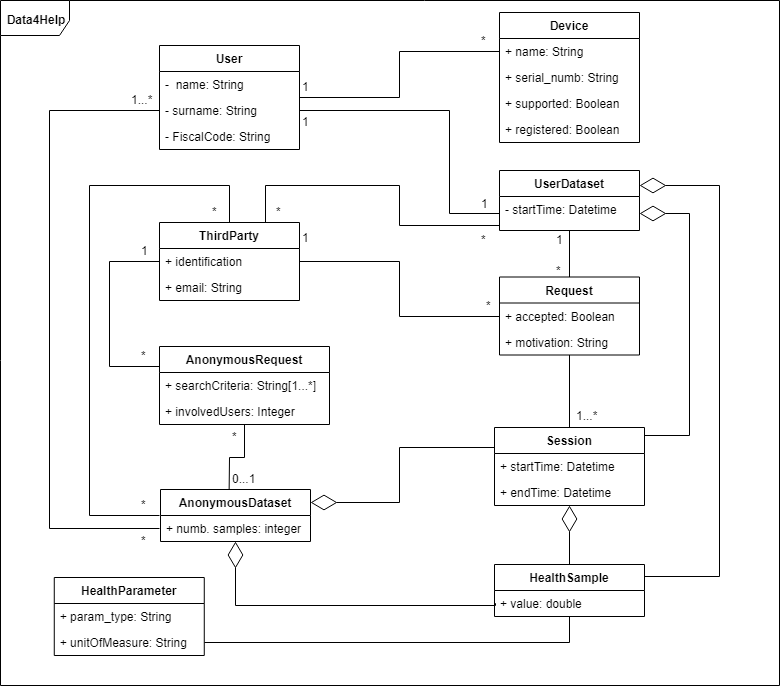
\includegraphics[scale=0.5]{Images/UML/D4H_class.png}
	\caption{Data4Help Class Diagram}
	\label{figure11}
\end{figure} 
\paragraph{}
As in the previous case a diagram can clarify the AutomatedSOS perspective:

\begin{figure}[H]
	\centering\setlength{\captionmargin}{0pt}%
	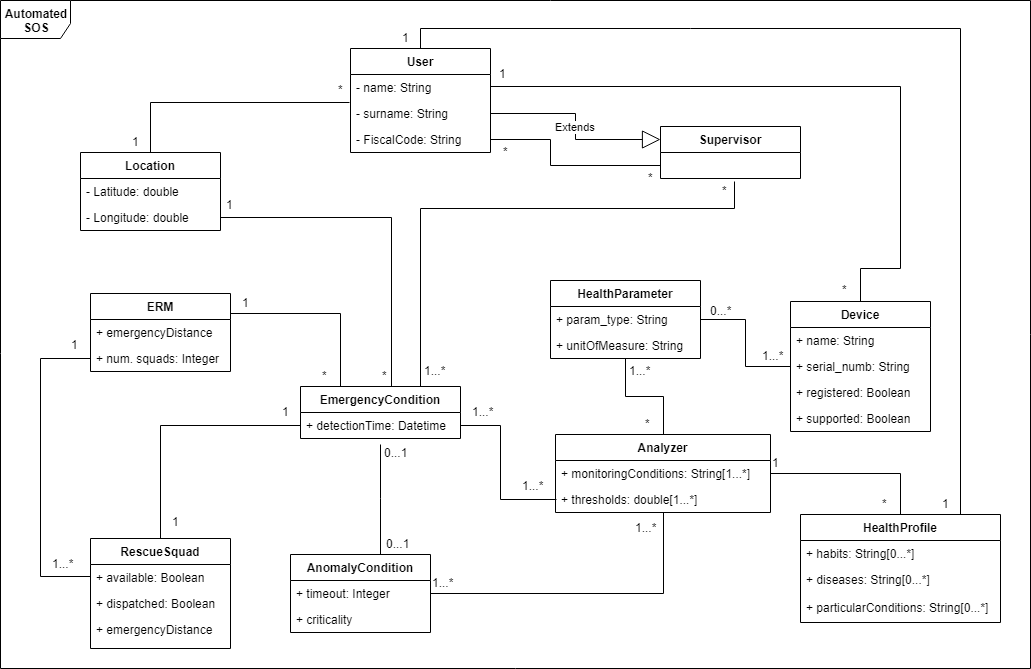
\includegraphics[scale=0.5]{Images/UML/ASOS_class.png}
	\caption{AutomatedSOS Class Diagram}
	\label{figure11}
\end{figure}



{\color{Blue}{\subsection{Product Functions}}}
{\color{Blue}{\subsubsection{Data4Help}}}
The main goal of Data4Help is to guarantee control on the health parameters of the users in order to give the possibility to third parties to obtain the data. Every user registered in Data4Help knows that his/her registered parameters could be used for market information, but also for helping researchers to discovers new treatments. This is made possible by providing two types of registration: the registration as a user and the registration as a third party.\\
There will be the possibility for the users to accept or deny personal requests from third parties, in this way there will be no privacy violations. On the other hand, the system will allow third parties to formulate anonymous requests. These are intended to not disclose the identity of the user, providing information of an heterogeneous set of users according to several requestor-specified search criteria. Unfortunately, it is trivial for a third party to trace back to sensitive information of a user providing restricting search parameters. After an attempt analysis, TrackMe evaluated a policy to prevent this possibility: in order to provide the result of an anonymous request to a third party, the involved users must be at least 1000. 
 %On the other hand, every request from the third party that comprehend at least 1000 of anonymous users will not require the consultation of every single user involved.\\
 %in order to control user’s parameters is possible to connect to the service various types of sensor devices.\\
 
\newpage
{\color{Blue}{\subsubsection{AutomatedSOS}}}
AutomatedSOS wants the users to feel safe. Provided the necessary sensor devices, the system guarantee a constant control on the health parameters. 
In order to minimize medical resource wasting, it is necessary for the system to discriminate carefully which conditions may lead to a fatality (e.g: heart attack) from those which can be simply false positive detections, uncareful behaviors of the person who is using the service, non-serious injuries or ambiguous observations. To this end, the system will be able to detect emergency and anomaly conditions.
%\begin{itemize}
	%\item \textit{Emergency Conditions}: unambiguous detections triggered by so-called critical events (e.g: heart attack)
	%\item \textit{Anomaly Conditions}: ambiguous detections that expect a reaction of the user and can be turned into emergencies under certain conditions
%\end{itemize}
%Every alteration that could possibly lead to an emergency is immediately notified to the user that could confirm the emergency condition or deny it. Alteration that are definitely sign of emergency lead immediately to an ambulance call.\\
Obviously, in order to guarantee that the number of false positives remains as low as possible, the user is required to give correct health information when he/she registers to the service. Furthermore the system will not allow a user to choose arbitrarily which set of sensor types will be used to monitor his/her health conditions. For each specific disease selected, there will be a set of specific sensor devices required.\\ 
The system will also provide the possibility to accept supervisors. This particular characters are AutomatedSOS users concepted to be supported by the system for giving assistance to other ones designated as supervised. Each time an AutomatedSOS users is in danger the system will be able to provide to the designated supervisor the necessary information. In this way, in case of emergency, there will be someone promptly informed.\\
As is known that it is not always possible to be monitored by the system, there is the possibility to notify the latter that it has to stop controlling the user parameters by turning off the service. The system also stops controlling them when the minimum required sensors are not available (maybe because they run out of battery), sending a notification to the user.  

{\color{Blue}{\subsubsection{Requirements}}}
\textbf{Data4Help}
\begin{itemize}
\item\textbf{[R1]:} The system must allow a registered user to associate a sensor device to the service
\item\textbf{[R2]:} Each user is uniquely identified by the system
\item\textbf{[R3]:} The system can acquire health data by specific sensors connected to the user's main device
\item\textbf{[R4]:} The system must be able to identify and certificate the reliability of each organization that wants to request user data
\item\textbf{[R5]:} Each registered organization that wants to access health data of specific users must be able to formulate a request providing information related to the purpose of the request.
\item\textbf{[R6]:} The system must notify each user of a third party request as soon as it is formulated, and allow him/her to accept or reject the request
\item\textbf{[R7]:} For each third party request the system should provide to the user information related to the requester and the purpose of the request
\item\textbf{[R8]:} Once a third party request is accepted by the user, the third party must have full access to the entire collection of data of the user
\item\textbf{[R9]:} Third parties must be able to request health data of groups of anonymous users, according to several criteria without being expressively authorized
\item\textbf{[R10]:} The system must prevent third parties to trace back to specific user information through anonymous requests
\end{itemize}
\paragraph{}
\textbf{AutomatedSOS}
\begin{itemize}
\item\textbf{[R11]:} The system must give the possibility to the user to specify him/her health profile
\item\textbf{[R12]:} The system must prevent the possibility to use the service, if the minimum required sensors are missing
\item\textbf{[R13]:} The system must allow the user to turn on and off the service each time he/she wants
\item\textbf{[R14]:} The system must stop monitoring when minimum required sensors are missing
\item\textbf{[R15]:} The system must be able to distinguish and detect emergency or anomaly conditions occurring to a specific user
\item\textbf{[R16]:} When an anomaly condition is detected, the system must send a notification to the user, asking if it is an emergency condition. If the user does not answer the notification within 30 seconds, the anomaly must become an emergency
\item\textbf{[R17]:} When an emergency condition is detected, the nearest ambulance must be alerted, providing all the information about the situation
\item\textbf{[R18]:} A user must have the possibility to request to become Supervisor of another one
\item\textbf{[R19]:} Each supervised user must be able to accept or reject the possibility to have a Supervisor
\item\textbf{[R20]:}The Supervisor must be notified by the system of all emergency and anomaly conditions occurring to the supervised user
\end{itemize}

\paragraph{}
{\color{Blue}{\subsection{User Characteristics}}}

%In both, Data4Help and AutomtedSOS the main actor is who we already called User. He/She is the one that provides health information to TrackMe while is monitored after the registration to the service. Without this presence, the application does not have any reason to exist.\\
%In a first hypothesis, the idea was to offer AutomatedSOS services only to elderly people. A more deep consideration of the provided service lead to the decision of permit to everyone that needs help to access to the application. A lot of young people need to be monitored as well as older one.\\

%Only in Data4Help there is the presence of another actor: the Third Party. It looks for the information provided by the users for its own interests (from business to healthcare). Third parties can access to the service if and only if they can provide a certification about who they are.


In Data4Help the main actor is who we already called User. He/She is the one that provides health information to TrackMe while is monitored after the registration to the service. Without this presence, the application does not have any reason to exist. He/She is uniquely recognizable by his/her fiscal code and his/her login information.There is also the presence of another actor: the Third Party. It looks for the information provided by the users for its own interests (from business to healthcare). Third parties can access to the service if and only if they can provide a certification about who they are. Without a valid certification the system denies the registration.\\
For what concerns AutomatedSOS and the Users of the application, in a first hypothesis the idea was to offer AutomatedSOS services only to elderly people. A more deep consideration of the provided service led to the decision to permit to everyone that needs help to access to the application. A lot of young people need to be monitored as well as older one.
\newpage

{\color{Blue}{\subsection{Assumptions, Dependencies and Constraints}}}
{\color{Blue}{\subsubsection{Domain Assumptions}}}
\raggedright
\textbf{Common Assumptions}
\begin{itemize}
	\item\textbf{[D1]:} The device to be registered, is supported by the system
	\item\textbf{[D2]:} The user is provided with a unique identification code (such as the Fiscal Code) that allows the system to associate him/her to a real person.
	\item\textbf{[D3]:} Data acquired by the connected sensors or directly provided by the user is intended to be accurate
	\item\textbf{[D4]:} The channel for the communication between the user and the system is reliable
\end{itemize}

\textbf{Data4Help}
\begin{itemize}
	\item \textbf{[D5]:} The system has access to external resources (e.g: existing companies database) required to allow authentication and reliability evaluation of all the third parties
	\item \textbf{[D6]:} The purpose of the request provided by the third party is intended to be truthful and accurate 
\end{itemize}
\textbf{AutomatedSOS}

\begin{itemize}
	\item\textbf{[D7]:} The user is registered to Data4Help
	\item\textbf{[D8]:} There is at least one hospital provided with an available ERM system (Emergency Resource Manager) 
	\item\textbf{[D9]:} The position of both the ambulance and the user is accurate
	\item\textbf{[D10]:} The Supervisor is a Data4Help registered user
	\item\textbf{[D11]:} The Supervisor is available when the notification is sent
\end{itemize}
\newpage

%------------------------------------------------------------------------------------------------------------------------------------------------
\clearpage
{\color{Blue}{\section{Specific Requirements}}}
\label{sect:requirements}
{\color{Blue}\subsection{External Interface Requirements}}
%\subsection{External Interface Requirements}
{\color{Blue}\subsubsection{D4H: User Interfaces}}
%\subsubsection{D4H: User Interfaces}

	
\begin{figure}[H]
	\centering
	\begin{minipage}[c]{.45\textwidth}
		\centering\setlength{\captionmargin}{0pt}%
		\fbox{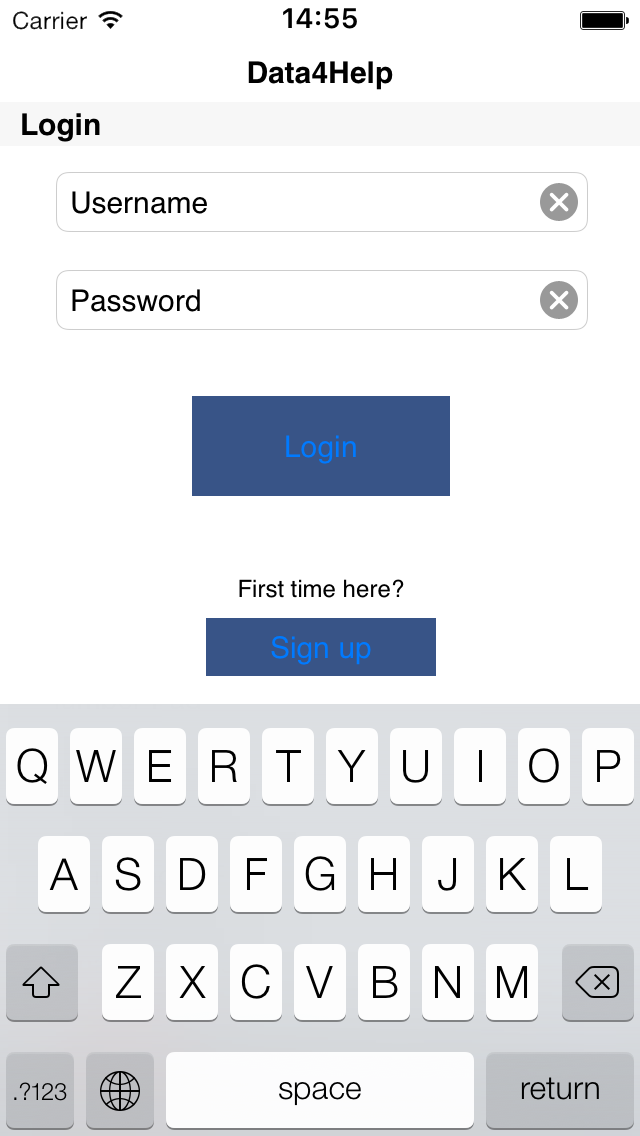
\includegraphics[scale=0.4]{Images/interfaces/Login.png}}
		\caption{User Login}
		\label{figura1}
	\end{minipage}%
	\hspace{5mm}%
	\begin{minipage}[c]{.45\textwidth}
		\centering\setlength{\captionmargin}{0pt}%
		\fbox{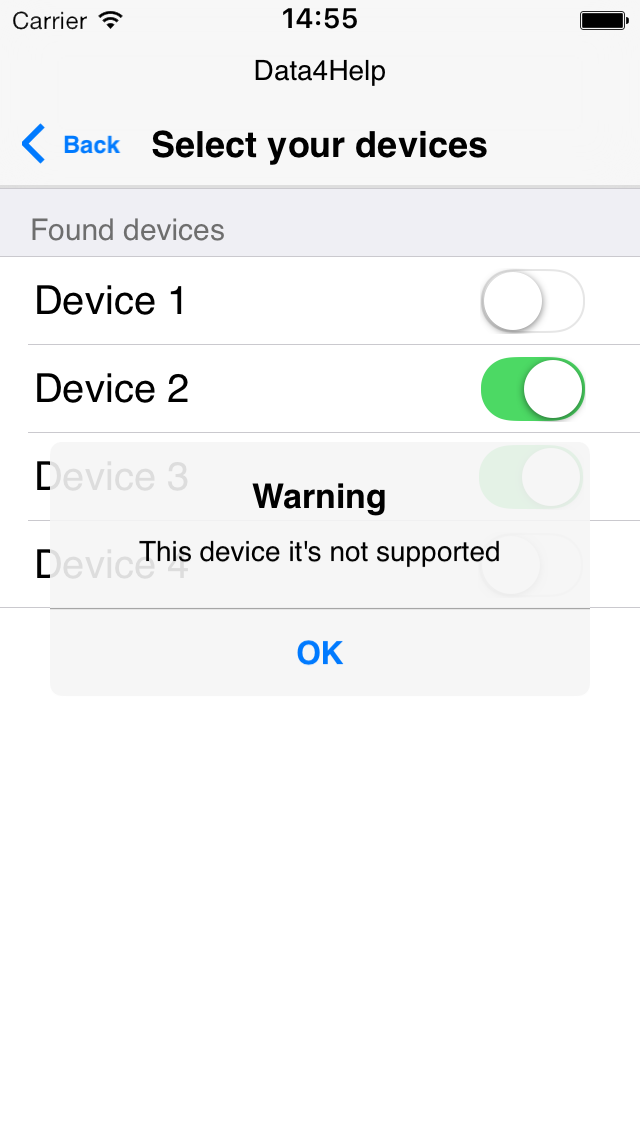
\includegraphics[scale=0.4]{Images/interfaces/SelectDevice.png}}
		\caption{Device not supported}
		\label{figura2}
	\end{minipage}
\end{figure}

\begin{figure}[H]
	\centering
	\begin{minipage}[c]{.45\textwidth}
		\centering\setlength{\captionmargin}{0pt}%
		\fbox{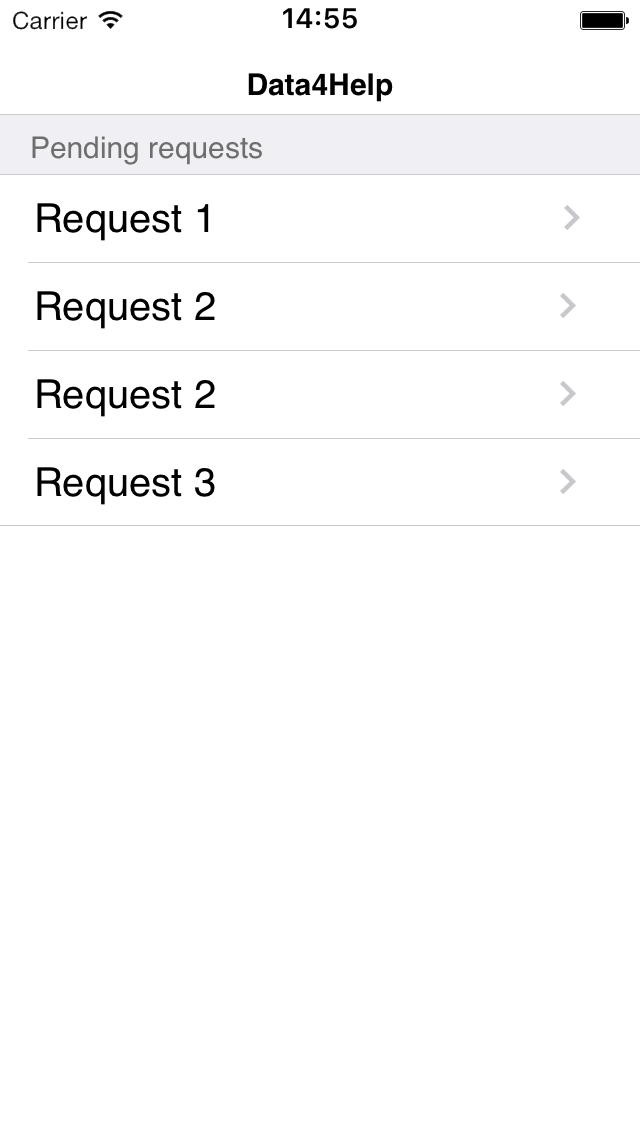
\includegraphics[scale=0.4]{Images/interfaces/PendingRequests.png}}
		\caption{Pending TP requests}
		\label{figura3}
	\end{minipage}%
	\hspace{5mm}%
	\begin{minipage}[c]{.45\textwidth}
		\centering\setlength{\captionmargin}{0pt}%
		\fbox{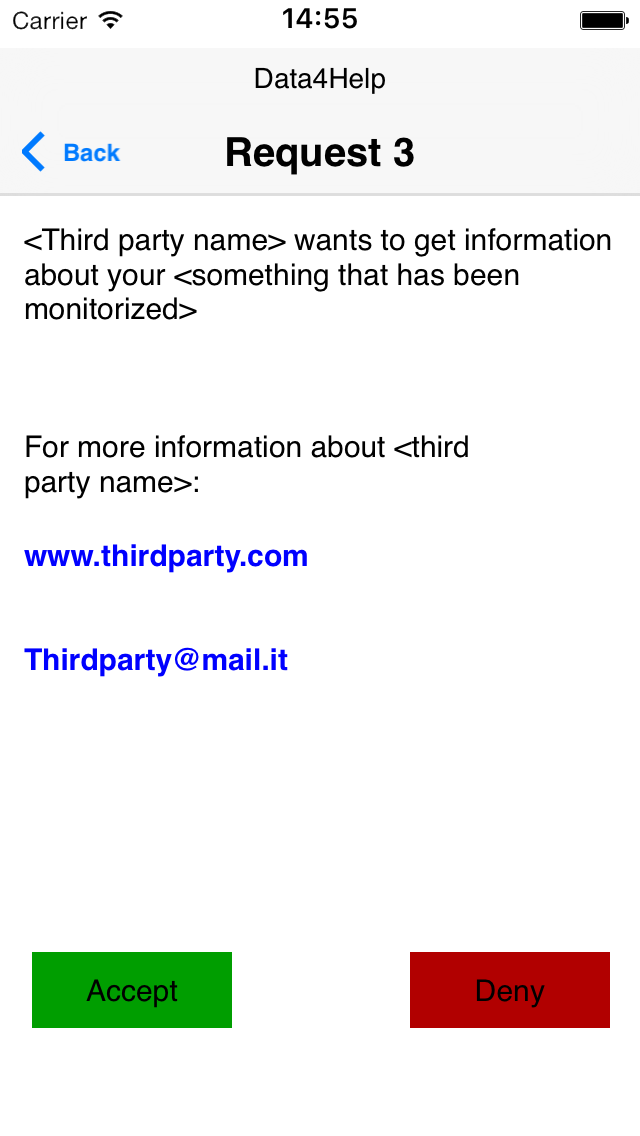
\includegraphics[scale=0.4]{Images/interfaces/TPRequest.png}}
		\caption{Evaluate Request}
		\label{figura4}
	\end{minipage}
\end{figure}

%\subsubsection{D4H: Third Party Interfaces}
{\color{Blue}\subsubsection{D4H: Third Party Interfaces}}
\begin{figure}[H]
	\centering
	\centering\setlength{\captionmargin}{0pt}%
	\fbox{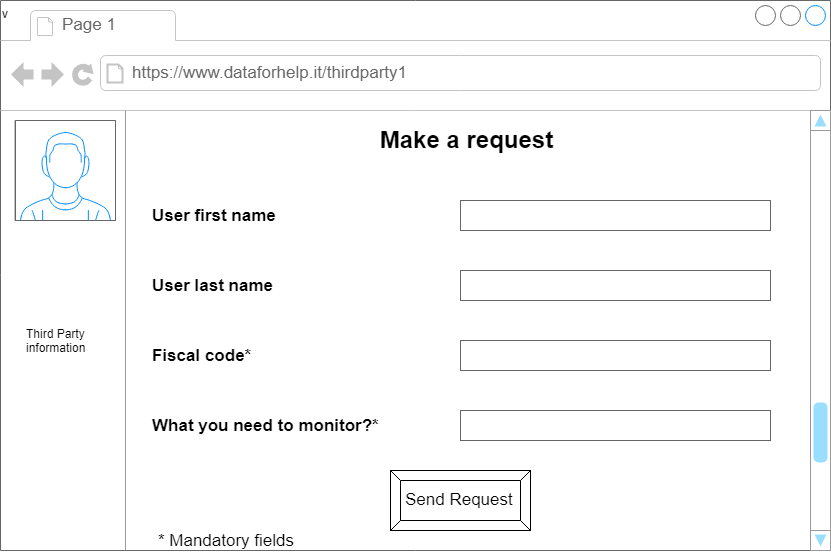
\includegraphics[scale=0.4]{Images/interfaces/MakeRequest.png}}
	\caption{TP make a request}
	\label{figura5}
\end{figure}

\begin{figure}[H]
	\centering\setlength{\captionmargin}{0pt}%
	\fbox{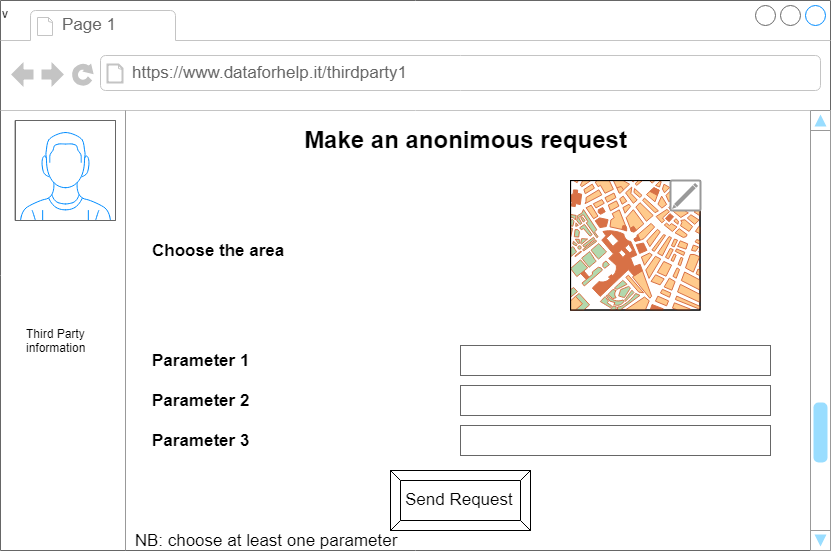
\includegraphics[scale=0.4]{Images/interfaces/AnonymousRequest.png}}
	\caption{TP make an anonymous request}
	\label{figura6}
\end{figure}

%\subsubsection{ASOS User Interfaces}
{\color{Blue}\subsubsection{ASOS User Interfaces}}

\begin{figure}[H]
	\centering
	\begin{minipage}[c]{.45\textwidth}
		\centering\setlength{\captionmargin}{0pt}%
		\fbox{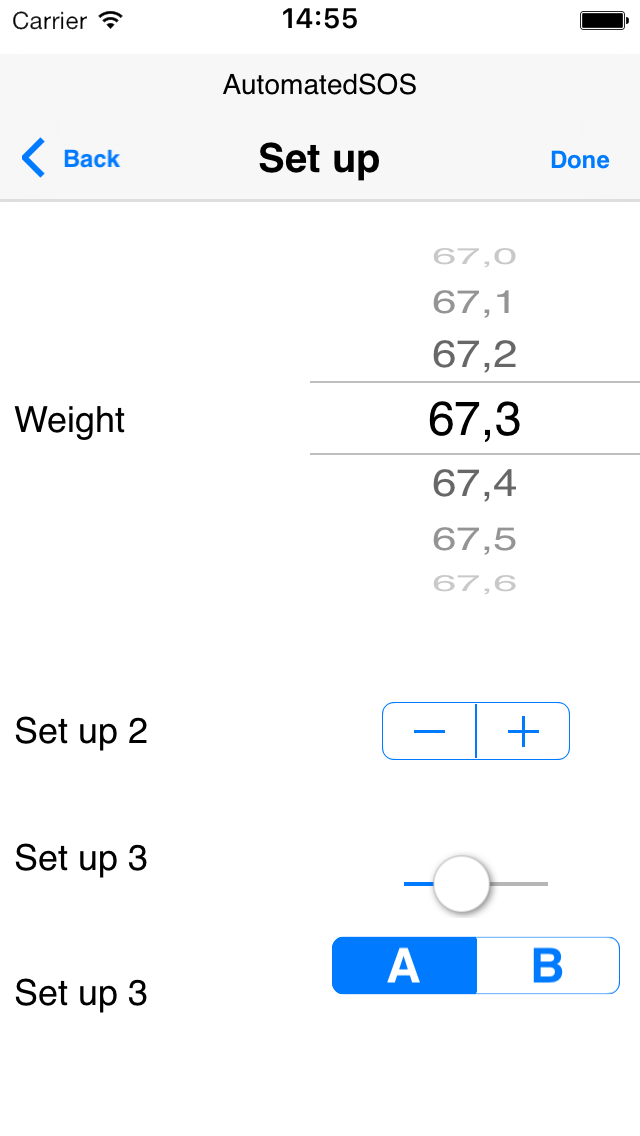
\includegraphics[scale=0.4]{Images/interfaces/Setup.png}}
		\caption{User Health Profile part 1}
		\label{figura7}
	\end{minipage}%
	\hspace{5mm}%
	\begin{minipage}[c]{.45\textwidth}
		\centering\setlength{\captionmargin}{0pt}%
		\fbox{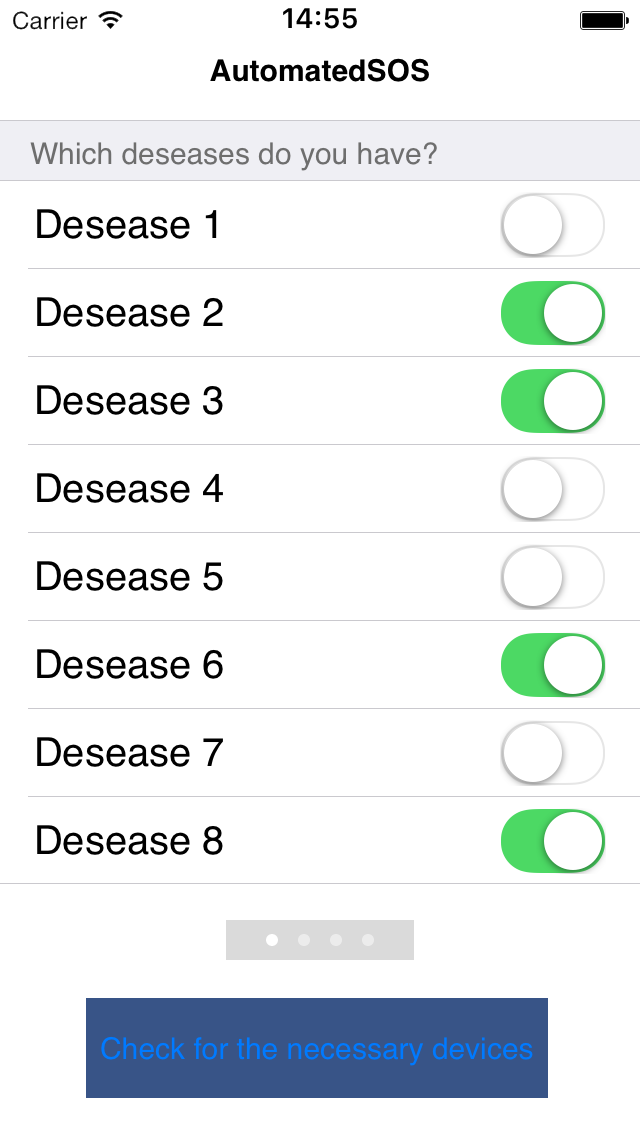
\includegraphics[scale=0.4]{Images/interfaces/SelectDesease.png}}
		\caption{User Health Profile part 2}
		\label{figura8}
	\end{minipage}
\end{figure}

\begin{figure}[htbp]
	\centering
	\begin{minipage}[c]{.45\textwidth}
		\centering\setlength{\captionmargin}{0pt}%
		\fbox{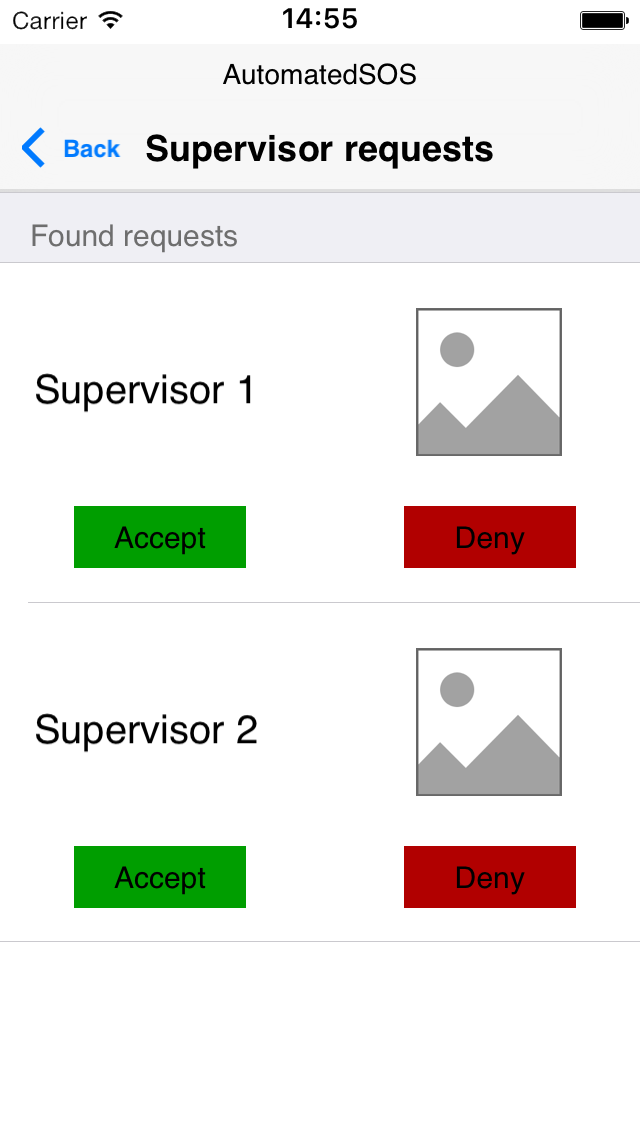
\includegraphics[scale=0.4]{Images/interfaces/Screen.png}}
		\caption{Supervisor Invitation}
		\label{figura9}
	\end{minipage}%
	\hspace{5mm}%
	\begin{minipage}[c]{.45\textwidth}
		\centering\setlength{\captionmargin}{0pt}%
		\fbox{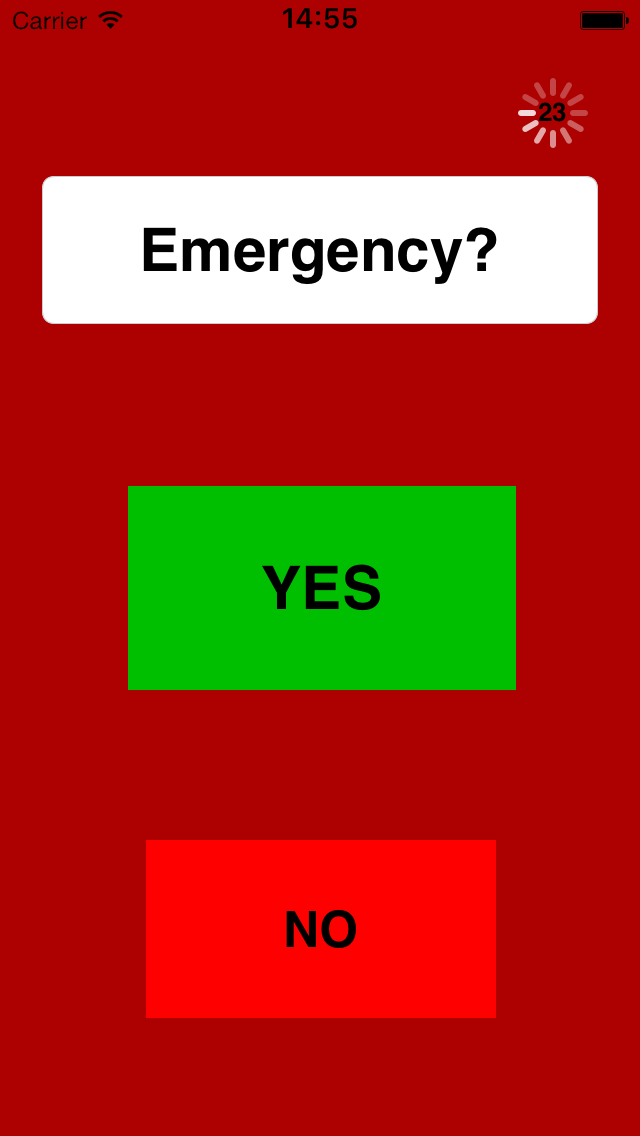
\includegraphics[scale=0.4]{Images/interfaces/EmergencyDetection.png}}
		\caption{Anomaly Detection}
		\label{figura10}
	\end{minipage}
\end{figure}
%\subsubsection{Hardware Interfaces}
{\color{Blue}\subsubsection{Hardware Interfaces}}
In order to work well and give the possibility to take advantage of the services offered by the system, both Data4Help and AuomatedSOS are required to be installed in a smartphone that provides:
\begin{itemize}
	\item GPS system
	\item Bluetooth (or BLE) interface
\end{itemize} 
The first requirement is needed especially for ASOS users, as substitute of GPS bracelets or similar, in order to provide the position of the user each time the system asks for it.\par
The second requirement is important because most of the available sensor devices on the market can be connected to the smartphone using Bluetooth or BLE interfaces.\par
Sensor devices are not mandatory but strongly suggested to allow D4H to acquire health parameters (like blood pressure, HR, breath rate and so on), without them, the application does not provide consistent advantages to the users. 
\paragraph{}


%\subsubsection{Software Interfaces}
{\color{Blue}\subsubsection{Software Interfaces}}
D4H and ASOS rely only on Google Maps API as external service. Both the computation and the storage part of the system are completely hosted and managed by TrackMe. Depending on more external services can affect negatively the reliability of the system. \par
\paragraph{}


%\subsubsection{Communication Interfaces}
{\color{Blue}\subsubsection{Communication Interfaces}}
In order to ensure confidentiality, data integrity and server authenticity, HTTPS is likely to be used as network protocol to manage the encrypted communication between the client (user or third party) and TrackMe servers for security reasons. Since the protocol uses TCP at transport layer is probable to deal with problems related to delays in communication. A deep analysis of how much acceptable are such delays must be carried out.
\paragraph{}



%\subsection{Data4Help Scenarios}
{\color{Blue}\subsection{Data4Help Scenarios}}
%\subsubsection{Scenario 1}
{\color{Blue}\subsubsection{Scenario 1}}

Ross is a Dr. Herbert's patient, he discovers that he is registered to Data4Help, the new service provided by TrackMe and decides to subscribe to it in order to facilitate the doctor to access his own health indicators. Ross so, downloads the app on his smartphone, runs it and fullfils the form for the registration. The system asks Ross the permission to collect data from all the devices the user will register in the system. Once this procedure is completed, the service detects that a compatible smartwatch and a respiratory rate monitoring device are connected to the mobile phone through the bluetooth interface. Then, the application asks Ross which one he wants to register to the service. Ross selects them and allow the system to complete the operation. The app, once finished, signals to the user that it is ready to notify possible requests from third parties to access the monitored information.
During the evening, Dr. Herbert receives the message from Ross who confirms his registration to Data4Help. The doctor logs in the service using the hospital credencials and inserts "Ross Gilbert" in the search form. Dr. Herbert then, once the system found the user's account, formulates the request including the motivation and sends it to Data4Help. Ross, the morning after, runs the application that notifies him of the awaiting request, so he checks for the requestor and accepts it.  
\paragraph{}

%\subsubsection{Scenario 2}
{\color{Blue}\subsubsection{Scenario 2}}

Angelo has bought two smart devices, an elastic strip equipped with a sensor able to measure blood pressure and an electronic bracelet for monitoring HR. He discovers that they can be interfaced with his smartphone through Bluetooth interface, so requests to the application to register the device, the service starts to check if the detected sensors are compatible or not. Unfortunately, only one of them is completely supported by the system: the sensor strip. So Angelo accepts to register only one device and the app, once performed the operation, update its status and return to collect data from all the connected devices.
\paragraph{}


%\subsubsection{Scenario 3}
{\color{Blue}\subsubsection{Scenario 3}}

SoftGalaxy is a software company that is working on a new application to provide to registered users a modern service called Health Advisor. It can suggest changes in daily habits, in diet and more, according to user data provided to the system. Unfortunately, the company cannot afford a large-scale system to collect information in real-time. In order to save as much resources as possible, it decides to rely on Data4Help to achieve this task. Before releasing the application, SoftGalaxy connects to the system and registers itself as third party, fulfilling the proper form. In addition, Data4Help asks the company to provide its digital certification for security reasons. Once the procedure is completed, the organization confirms the registration through the company's email address. 
\paragraph{}


%\subsubsection{Scenario 4}
{\color{Blue}\subsubsection{Scenario 4}}
The company Virgin Active is considering opening a new gym near Saint Ambrogio church in Milan. In order to do so, it decides to ask to Track Me to receive the information about all the overweight people that live in the area of Saint Ambrogio. TrackMe replied with a negative answer because there are only 593 people that suits with the requirements. Virgin Active has to change the request and so asks the same information but for a larger area taking in also the area of Saint Agostino. This time there are enough people to let the request being forwarded and so Virgin Active can receive the information needed.
\paragraph{}


%\subsection{AutomatedSOS Scenarios}
{\color{Blue}\subsection{AutomatedSOS Scenarios}}
%\subsubsection{Scenario 1}
{\color{Blue}\subsubsection{Scenario 1}}
Michelle has an elderly mother, Teresa, who suffers about a rare heart disease. She is constantly monitored by a portable ECG device due to the high risk of being hit by an heart attack. Unfortunately, Michelle works during the morning and in this period of the day no one takes care of Teresa. She suggests to the mother to rely on AutomatedSOS, a Data4Help-based service. Since the elderly woman has a smartphone, with Data4Help installed and a personal account, she decides to download the application and logs in with Data4Help credencials. The system notices that Teresa is using the service for the first time, so it asks some information about her health problems and through it the app creates an health profile and a list of required sensors. The ECG that is actually monitoring her, is already registered and used by Data4Help, but since she has specified that suffers about loss of consciousness the system warns her that a fall sensor should be registered to provide the proper assistance. Teresa has not the device yet, so ignores the warning and complete the profiling procedure. The app finally, is ready to monitor the woman’s health status.
\paragraph{}


%\subsubsection{Scenario 2}
{\color{Blue}\subsubsection{Scenario 2}}
Marianna  turned  60  one  month  ago  and  recieved  a  notification  from the  app  Data4Help  that  prouposed  her  to  join  to  asos.  She  decided  that  it  could  be  a  good  idea  in  order  to  live  better  and  safer.  As  soon  as  she  acceptend  to  join  it,  Marianna  is  aked  to  fill  a  questionnaire  about  some  basic  information  of  herself.  A  few  days  after,  she  had  dinner  with  friends  and  ordered  a  piece  of  cake  without  knowing  that  inside  it  there  were  almonds,  a  food  that  gaves  her  anaphylactic  shock.  Immediately  she  started  to  breath  bad,  her  heartbeat  increased  and  also  her  pressure.  Her  phone  rung,  asos  was  asking  if  everything  was  ok.  As  Marianna  needed  an  ambulance,  she  answered  negatively.  Her  husband received a notification from asos that Marianna was sick and an ambulance arrived at the restaurant, saving Marianna.   
\paragraph{}


%\subsubsection{Scenario 3}
{\color{Blue}\subsubsection{Scenario 3}}
Carol is a young student, she is subjected to loss of consciousness episodes due to medicines she has to take for a congenital disease. Carol is an ASOS user as well as her mother, Jenny. This last one decides to watch over the health conditions of her daughter when she is outside home. So, Jenny in order to be notified of all the emergencies and provides support when near the daughter, opens AutomatedSOS and sends to Carol an invitation for becoming her Supervisor. Carol, during the school break receives the request and accepts it. Becoming a Supervisor, Jenny is allowed to be notified of the daughter health status when something goes wrong and to know the position of Carol.
\paragraph{}


%\subsection {Functional Requirements}
{\color{Blue}\subsection{Functional Requirements}}

%\subsubsection{Data4Help}
{\color{Blue}\subsubsection{Data4Help}}

\textbf{G1: A user can register personal health monitoring devices in the system}
\begin{itemize}
	\item R1: The system must allow a registered user to associate a sensor device to the service
	\item D1: The device to be registered, is supported by the system.
\end{itemize}

\textbf{G2: TrackMe acquires periodically health parameters specifically related to a user.}
\begin{itemize}
	\item R2: Each user is uniquely identified by the system.
	\item R3: The system can acquire health data by specific sensors connected to the user's main device.
	\begin{itemize}
		\item D2.1: Data acquired by the connected sensors is intended to be accurate.
	\end{itemize}
	\item R4: The system must provide the possibility to users to insert specific health information that cannot be acquired through other monitoring devices.
	\begin{itemize}
		\item D2.2: Health information manually provided by the user is intended to be correct.
	\end{itemize}   
	
\end{itemize}
\textbf{G2.1: Third parties can access health data of specific users, if expressively authorized by the them}

\begin{itemize}
	\item R4: The system must be able to identify and certificate the reliability of each organization that wants to request user data
	\item R5: Each registered organization that wants to access health data of specific users must be able to formulate a request providing information related to the purpose of the request
	\item R6: The system must notify each user of a third party request as soon as it is formulated, and allow him/her to accept or reject the request
	\item R7: For each third party request the system should provide to the user, information related to the requestor and the purpose of the request
	\item R8: Once a request is accepted, a third party must have full access to all collected data of the user
\end{itemize}

\raggedright
\textbf{G2.2: Third-parties can request anonymous information about groups of people.}

\begin{itemize}
	\item R9: Third parties must be able to request health data of groups of anonymous users, according to several criteria without being expressively authorized.
	\item R10: The system must prevent third parties to trace it back to specific user information through anonymous requests.
\end{itemize}

%\subsubsection{AutomatedSOS}
{\color{Blue}\subsubsection{AutomatedSOS}}

\textbf{G1: The user has the possibility to specify the diseases he/she has, so the system can evaluate which health parameters monitorize.}

\begin{itemize}
	\item R1: The system must give the possibility to the user to specify which diseases he/she has.
	\begin{itemize}
		\item D1: The user is registered to AutomatedSOS.
	\end{itemize} 
	\item R2: The system must prevent the possibility to use the service, if the minimum required sensors are missing
\end{itemize}

\textbf{ G2: An ambulance may be sent within 5 seconds, if an emergency or anomaly condition is detected.}

\begin{itemize}
	\item R3: The system must be able to distinguish and detect emergency or anomaly conditions occurring to a specific user
	\item R4: When an anomaly condition is detected, the system must send a notification to the user, asking if it is an emergency condition.
	\item R5: When an emergency condition is detected, the nearest ambulance must be alerted, providing all the information about the situation.
	\begin{itemize}
		\item D2.1: The sensor devices monitoring the patient are providing reliable data.
		\item D2.2: The position of both the ambulance and the user are accurately provided by the GPS system.
	\end{itemize}
\end{itemize}

\textbf{G3: A user designated as Supervisor of another one, is notified of both emergency and anomaly events occuring to the supervised user.}

\begin{itemize}[itemsep=0em]
	\item R7: A user must be allowed by the system to become Supervisor of another one.
	\begin{itemize}
		\item D3.2: The Supervisor is a Data4Help registered user.
	\end{itemize}
	\item R8: Each supervised user must be able to accept or reject the possibility to have a Supervisor.
	\item R9: The Supervisor must be notified by the system of all emergency and anomaly conditions occurring to the supervised user.
	\begin{itemize}[topsep=0em]
		\item D3.1: The Supervisor is available when the notification is sent.
	\end{itemize}
\end{itemize}

%\subsection{UML Modeling}
{\color{Blue}\subsection{UML Modeling}}

%\subsubsection{Data4Help Use Cases}
{\color{Blue}\subsubsection{Data4Help Use Cases}}
\begin{table}[htb]
	\centering
	{\renewcommand{\arraystretch}{2}%
		\begin{tabular}{|@{\hspace{2em}} p{4cm} @{}| p{11cm} @{\qquad}| }
			\cline{1-2}
			\multicolumn{2}{|c|}{\textbf{User Signs Up}} \\ \cline{1-2}
			\textbf{Actors:} & User \\ \cline{1-2}
			\textbf{Entry Conditions:} & The user has already downloaded the application \\ \cline{1-2}
			\textbf{Flow of Events:} & 
			\begin{enumerate}[itemsep=-0.2em, topsep=0em]
				\item The user clicks on "Signs up as User"
				\item The user inserts all the required information
				\item The user confirms the registration
				\item The system asks the user if he/she wants to 
				associate a sensor device to the service.
				\item The user accepts to register the devices
				\item The system redirect the user to the Device Registration space
				\item The user \underline{registers the devices} connected to the smartphone
				\item The system redirect the user to his/her personal account
			\end{enumerate}\\ \cline{1-2}
			\textbf{ Conditions:} & The user is successfully signed up\\ \cline{1-2}
			\textbf{Exceptions:} & 
			\begin{itemize}[itemsep=-0.2em, topsep=0em]
				\item 3) The user is already registered to the service, a notification will be sent, preventing him/her to register again.
				\item 4) The user skips the device registration and the system redirect the user directly to his/her account
			\end{itemize} \\ \cline{1-2}
			\small{\textbf{Special Requirements:}} & None \\ \hline
	\end{tabular}} \quad
\end{table}

\begin{table}[H]
	\centering
	{\renewcommand{\arraystretch}{1.5}%
		\begin{tabular}{|@{\hspace{2em}} p{4cm} @{}| p{11cm} @{\qquad}| }
			\cline{1-2}
			\multicolumn{2}{|c|}{\textbf{User Login}} \\ \cline{1-2}
			\textbf{Actors:} & User \\ \cline{1-2}
			\textbf{Entry Conditions:} &  The user is already signed up \\ \cline{1-2}
			\textbf{Flow of Events:} &
			 \begin{enumerate}[itemsep=-0.2em, topsep=0em]
				\item The user inserts the access credencials
				\item The user taps on "Log in"
			\end{enumerate}\\ \cline{1-2}
			\textbf{Exit Conditions:} & The system redirect the user to his/her personal account\\ \cline{1-2}
			\textbf{Exceptions:} & 
			\begin{itemize}
				\item If the username or the password are incorrect the user is requested to rewrite them
			\end{itemize} \\ \cline{1-2}
			\textbf{Special Requirement:} & None\\ \cline{1-2}
	\end{tabular}} \quad
\end{table}

\begin{table}[htb]
	\centering
	{\renewcommand{\arraystretch}{1.5}%
		\begin{tabular}{|@{\hspace{2em}} p{4cm} @{}| p{11cm} @{\qquad}|}
			\cline{1-2}
			\multicolumn{2}{|c|}{\textbf{Register Device}} \\ \cline{1-2}
			\textbf{Actors:} & User \\ \cline{1-2}
			\textbf{Entry Conditions:} &  The user is logged in Data4Help \\ \cline{1-2}
			\textbf{Flow of Events:} &
			 \begin{enumerate}[itemsep=-0.2em, topsep=0em]
				\item The user taps on "Add Device"
				\item The system provides the list of all the sensor devices connected to the smartphone
				\item The user selects the devices he/she wants to associate to the service
				\item The system registers the devices
			\end{enumerate} \\ \cline{1-2}
			\textbf{Output Conditions:} & A new monitoring device is added in the system \\ \hline
			\textbf{Exceptions:} & 
			\begin{itemize}[itemsep=-0.2em, topsep=-2em, partopsep=-1em]
				\item If the registered sensor corresponds to a new monitored parameter the information is associated to the current user in the system 
				\item If the device is not supported, the system warns the user and denies the device registration.
			\end{itemize} \\ \cline{1-2}
			\textbf{Special Requirement:} & None \\ \hline
	\end{tabular}} \quad
\end{table}

\begin{table}[H]
	\centering
	{\renewcommand{\arraystretch}{1.5}%
		\begin{tabular}{|@{\hspace{2em}} p{4cm} @{}| p{11cm} @{\qquad}|}
			\cline{1-2}
			\multicolumn{2}{|c|}{\textbf{ThirdParty Sign Up}} \\ \cline{1-2}
			\textbf{Actors:} & Third Party \\ \cline{1-2}
			\textbf{Entry Conditions:} & The third party has not registered to the service yet \\ \cline{1-2}
			\textbf{Flow of Events:} & 
			\begin{enumerate}[itemsep=-0.2em, topsep=0em]
				\item The third party clicks on "Sign Up as Third Party"
				\item The third party inserts the requested information
				\item The third party provides a certification of its identity
				\item The third party confirms the information provided
				\item The system verifies the inserted data
				\item The system confirms the registration and redirect the third party to its personal account.
			\end{enumerate}\\ \cline{1-2}
			\textbf{Exit Conditions:} & The third party is registered to Data4Help \\ \hline
			\textbf{Exceptions:} & 
			\begin{itemize}[itemsep=-0.2em, topsep=0em]
				\item If the information provided is incorrect or the third party is already registered, the system shows a warning and denies the registration
			\end{itemize} \\ \hline
			\textbf{Special Requirements:} & None\\ \hline
	\end{tabular}} \quad
\end{table}

\begin{table}[H]
	\centering
	{\renewcommand{\arraystretch}{1.5}%
		\begin{tabular}{|@{\hspace{2em}} p{4cm} @{}| p{11cm} @{\qquad}|}
			\cline{1-2}
			\multicolumn{2}{|c|}{\textbf{ThirdParty Logs in}} \\ \cline{1-2}
			\textbf{Actors:} & Third Party \\ \cline{1-2}
			\textbf{Entry Conditions:} & The third party is already registered in the service \\ \cline{1-2}
			\textbf{Flow of Events:} & \begin{enumerate}[topsep=0em, itemsep=-0.2em]
				\item The third party clicks on "Log in as Third Party"
				\item The third party inserts the access credencials
				\item The system verifies the provided information
			\end{enumerate}\\ \cline{1-2}
			\textbf{Exit Conditions:} & the system redirects the third party to its personal account\\ \cline{1-2}
			\textbf{Exceptions:} & \begin{itemize}
				\item If the credencials inserted are not valid, the system sends a warning and denies the access
			\end{itemize} \\ \cline{1-2}
			\textbf{Special Requirements:} & None \\ \cline{1-2}
	\end{tabular}} \quad
\end{table}

\begin{table}[H]
	\centering
	{\renewcommand{\arraystretch}{1.5}%
		\begin{tabular}{|@{\hspace{2em}} p{4cm} @{}| p{11cm} @{\qquad}|}
			\cline{1-2}
			\multicolumn{2}{|c|}{\textbf{Make a Request}} \\ \cline{1-2}
			\textbf{Actors:} & Third Party \\ \cline{1-2}
			\textbf{Entry Conditions:} &  The third party has already signed up for D4H  \\ \cline{1-2}
			\textbf{Flow of Events:} & 
			\begin{enumerate}[itemsep=-0.2em, topsep=0em]
				\item The third party clicks on "Create Request"
				\item The third party selects the user data types that wants to access and inserts the information required to find the user
				\item The third party provides the motivation of the request.
				\item The system checks if someone matches the search criteria and provide the result
				\item The third party clicks on "Send Request"
				\item The system notifies the third party that the request has been sent to the user
			\end{enumerate}\\ \cline{1-2}
			\textbf{Exit Conditions:} & The request is sent to the specific user\\ \cline{1-2}
			\textbf{Exceptions:} & 
			\begin{itemize}[topsep=-2em, itemsep=-0.2em]
				\item If the specified search criteria do not provide a valid result, the system shows a warning and the request is not created.
			\end{itemize} \\ \cline{1-2}
			\textbf{Special Requirements:} & The third party knows exactly the minimum search information required to find the specific user \\ \hline
	\end{tabular}} \quad
\end{table}

\begin{table}[H]
	\centering
	{\renewcommand{\arraystretch}{1.5}%
		\begin{tabular}{|@{\hspace{2em}} p{4cm} @{}| p{11cm} @{\qquad}|}
			\cline{1-2}
			\multicolumn{2}{|c|}{\textbf{Evaluate Request}} \\ \cline{1-2}
			\textbf{Actors:} & User \\ \cline{1-2}
			\textbf{Entry Conditions:} & \begin{itemize}[itemsep=-0.2em, topsep=0em]
				\item The user is logged in Data4help
				\item The user is notified by the system that a third party request has been received
			\end{itemize} \\ \cline{1-2}
			\textbf{Flow of Events:} & \begin{enumerate}[itemsep=-0.2em, topsep=0em]
				\item The user enters the pending requests
				\item The user selects the last request
				\item The user taps on the request 
				\item The system shows to the user identity and motivation of the requestor
				\item The user accepts the request
				\item The system notifies the third party about the decision of the user
			\end{enumerate} \\ \cline{1-2}
			\textbf{Exit Conditions:} & The system allows the third party to access the requested user's dataset\\ \cline{1-2}
			\textbf{Exceptions:} & 
			\begin{itemize}[itemsep=-0.2em, topsep=0em]
				\item If the user rejects the request, the system notifies the rejection to the third party
				\item If the request has been aborted by the third party or is expired  the system notifies the user that the request is no longer acceptable or rejectable
			\end{itemize} \\ \cline{1-2}
			\textbf{Special Requirements: } & None \\ \hline
	\end{tabular}} \quad
\end{table}

\begin{table}[H]
	\centering
	{\renewcommand{\arraystretch}{1.5}%
		\begin{tabular}{|@{\hspace{2em}} p{4cm} @{}| p{11cm} @{\qquad}|}
			\cline{1-2}
			\multicolumn{2}{|c|}{\textbf{Make an Anonymous Request}} \\ \cline{1-2}
			\textbf{Actors:} & Third party \\ \cline{1-2}
			\textbf{Entry Conditions:} & The third party is logged in Data4Help \\ \cline{1-2}
			\textbf{Flow of Events:} & 
			\begin{enumerate}[itemsep=-0.2em, topsep=0em]
				\item The third party clicks on "Create Anonymous Request"
				\item The third party specifies the search criteria required to find the group of anonymous users
				\item The system checks if number of involved anonymous users are at least 1000, according the search criteria
				\item The system notifies the requestor that a valid dataset has been found
			\end{enumerate}\\ \cline{1-2}
			\textbf{Exit Conditions:} & The third party obtains the anonymous dataset \\ \cline{1-2}
			\textbf{Exceptions:} & 
			\begin{itemize} [itemsep=-0.2em, topsep=0em]
				\item 3) If the anonymous users involved in the request are less than 1000 or no one matches the search criteria, the system notifies the event and rejects the request.
			\end{itemize} \\ \cline{1-2}
			\textbf{Special Requirements:} & None \\ \hline
	\end{tabular}} \quad
\end{table}


\begin{center}
	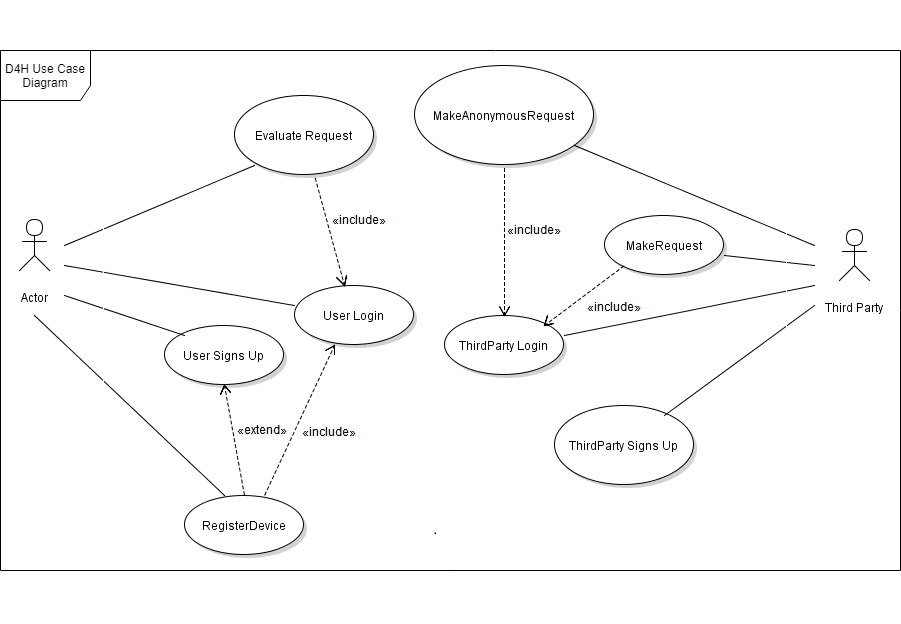
\includegraphics[scale=1.1]{Images/UML/D4H_usecase.png}
\end{center}

%\subsubsection{AutomatedSOS Use Cases}
{\color{Blue}\subsubsection{AutomatedSOS Use Cases}}

\begin{table}[H]
	\centering
	{\renewcommand{\arraystretch}{1.5}%
		\begin{tabular}{|@{\hspace{2em}} p{4cm} @{}| p{11cm} @{\qquad}|}
			\cline{1-2}
			\multicolumn{2}{|c|}{\textbf{User Logs in ASOS}} \\ \cline{1-2}
			\textbf{Actors:} & User \\ \cline{1-2}
			\textbf{Entry Conditions:} & The user is already registered in Data4Help \\ \cline{1-2}
			\textbf{Flow of Events:} & \begin{enumerate}[topsep=0em, itemsep=-0.2em]
				\item The user inserts the D4H access credencials
				\item The user clicks on "Log in"
				\item The system checks if the credencials are valid
			\end{enumerate}\\ \cline{1-2}
			\textbf{Exit Conditions:} & The system redirects the user to his/her personal ASOS account\\ \cline{1-2}
			\textbf{Exceptions:} & \begin{itemize}[topsep=0em, itemsep=-0.2em]
				\item If the user inserts wrong credencials the system sends a warning and denies the access
				\item If the user has logged in for the first time, the system starts to \underline{profile the health conditions of the user} (see:"Change User Health Profile")
			\end{itemize} \\ \cline{1-2}
			\textbf{Special Requirements:} & None \\ \cline{1-2}
	\end{tabular}} \quad
\end{table}

\begin{table}[H]
	\centering
	{\renewcommand{\arraystretch}{1.5}%
		\begin{tabular}{|@{\hspace{2em}} p{4cm} @{}| p{11cm} @{\qquad}|}
			\cline{1-2}
			\multicolumn{2}{|c|}{\textbf{Change Health Profile}} \\ \cline{1-2}
			\textbf{Actors:} & User \\ \cline{1-2}
			\textbf{Entry Conditions:} & %% [topsep=0em, itemsep=-0.2em]
 The user is logged in for the first time \\ \cline{1-2}
			\textbf{Flow of Events:} & \begin{enumerate}[topsep=0em, itemsep=-0.2em]
				\item The user clicks on "Manage Health Profile"
				\item The user inserts personal information regarding age, daily habits, addictions, diagnosed diseases
				\item The system evaluates and provides a list of clinical conditions that can be monitored according to the inserted information
				\item The system checks if the sensors required for monitoring the given clinical conditions are registered to D4H and connected to the smartphone
				\item The user confirms the result 
			\end{enumerate} \\ \cline{1-2}
			\textbf{Exit Conditions:} & The health profile is updated and the user is monitored according to the new clinical conditions \\ \cline{1-2}
			\textbf{Exceptions:} & \begin{itemize}[topsep=0em, itemsep=-0.2em]
				\item 3) If none of the minimum required sensors are registered or connected, the system warns the user and denies the service.
				\item 3) If only a part of the required sensors (at least the minimum required ones) are registered in the service, the user selects which of the available clinical conditions he/she wants to be monitored and confirms.
				\end{itemize}  \\ \cline{1-2}
			\textbf{Special Requirements:} & None \\ \cline{1-2}
	\end{tabular}} \quad
\end{table}

\begin{table}[htb]
	\centering
	{\renewcommand{\arraystretch}{1.5}%
		\begin{tabular}{|@{\hspace{2em}} p{4cm} @{}| p{11cm} @{\qquad}|}
			\cline{1-2}
			\multicolumn{2}{|c|}{\textbf{Send Supervisor Request}} \\ \cline{1-2}
			\textbf{Actors:} & User \\ \cline{1-2}
			\textbf{Entry Conditions:} & The user is logged in ASOS \\ \cline{1-2}
			\textbf{Flow of Events:} & \begin{enumerate}[topsep=0em, itemsep=-0.2em]
				\item The user clicks on "Become Supervisor"
				\item The system asks the identification of who should be supevised
				\item The user inserts the fiscal code of the supervised user
				\item The system provides the result of the research
				\item The user sends the request
			\end{enumerate}\\ \cline{1-2}
			\textbf{Exit Conditions:} & The receiver is notified of the supervisor request\\ \cline{1-2}
			\textbf{Exceptions:} & \begin{itemize}
				\item 4) The research criteria do not match any existing ASOS user
			\end{itemize} \\ \cline{1-2}
			\textbf{Special Requirements:} & None \\ \cline{1-2}
	\end{tabular}} \quad
\end{table}
\begin{table}[H]
	\centering
	{\renewcommand{\arraystretch}{1.5}%
		\begin{tabular}{|@{\hspace{2em}} p{4cm} @{}| p{11cm} @{\qquad}|}
			\cline{1-2}
			\multicolumn{2}{|c|}{\textbf{Anomaly Condition is Detected}} \\ \cline{1-2}
			\textbf{Actors:} & User\\ \cline{1-2}
			\textbf{Entry Conditions:} & \begin{itemize}[topsep=0em, itemsep=-0.2em]
				\item The user is logged in AutomatedSOS
				\item The ASOS Monitor Mode is switched on
				\item ASOS system has detected an Anomaly Condition 
			\end{itemize} \\ \cline{1-2}
			\textbf{Flow of Events:} & \begin{enumerate}[topsep=0em, itemsep=-0.2em]
				\item The user is notified by the system that asks to him/her if an ambulance is needed 
				\item The user confirms that is a matter of emergency
				\item The system turns the anomaly into an emergency condition
			\end{enumerate}\\ \cline{1-2}
			\textbf{Exit Conditions:} & The system raises an \underline{emergency condition} (see:"An Emergency Condition is Detected")\\ \cline{1-2}
			\textbf{Exceptions:} & \begin{itemize}[topsep=0em, itemsep=-0.2em]
				\item The user is fine, he/she notifies the system that an ambulance is not required
				\item If the user does not reply to the notification, the anomaly timeout expires and the system alerts the nearest hospital
			\end{itemize} \\ \cline{1-2}
			\textbf{Special Requirements:} & The timeout must fixed to 30 seconds \\ \cline{1-2}
	\end{tabular}} \quad
\end{table}

\begin{table}[htb]
	\centering
	{\renewcommand{\arraystretch}{1.5}%
		\begin{tabular}{|@{\hspace{2em}} p{4cm} @{}| p{11cm} @{\qquad}|}
			\cline{1-2}
			\multicolumn{2}{|c|}{\textbf{Evaluate Supervisor Request}} \\ \cline{1-2}
			\textbf{Actors:} & User \\ \cline{1-2}
			\textbf{Entry Conditions:} & \begin{itemize}[topsep=0em, itemsep=-0.2em]
				\item The user is logged in ASOS
				\item The user is notified that a Supervisor request has been received
			\end{itemize} \\ \cline{1-2}
			\textbf{Flow of Events:} & \begin{enumerate}[topsep=0em, itemsep=-0.2em]
				\item The user enters the list of the pending supervisor requests
				\item The user selects the request
				\item The system provides the identity of the requestor
				\item The user accepts the request
			\end{enumerate}\\ \cline{1-2}
			\textbf{Exit Conditions:} & The system notifies the new Supervisor and allow him/her to access the user's health status and position during emergencies  \\ \cline{1-2}
			\textbf{Exceptions:} & \begin{itemize}
				\item 4) If the user rejects the request the system notifies the requestor of the refuse.
			\end{itemize} \\ \cline{1-2}
			\textbf{Special Requirements:} & None \\ \cline{1-2}
	\end{tabular}} \quad
\end{table}

\begin{table}[H]
	\centering
	{\renewcommand{\arraystretch}{1.5}%
		\begin{tabular}{|@{\hspace{2em}} p{4cm} @{}| p{11cm} @{\qquad}|}
			\cline{1-2}
			\multicolumn{2}{|c|}{\textbf{An Emergeny Condition is Detected}} \\ \cline{1-2}
			\textbf{Actors:} & EmergencyResourceManager \\ \cline{1-2}
			\textbf{Entry Conditions:} & \begin{itemize}[topsep=0em, itemsep=-0.2em]
				\item An emergency condition is detected.
				\item An anomaly is turned into an emergency condition
			\end{itemize} \\ \cline{1-2}
			\textbf{Flow of Events:} & \begin{enumerate}[topsep=0em, itemsep=-0.2em]
				\item The system sends an alert to the nearest hospital's ERM providing the identification and position of the user, the reason of the emergency, the time instant at which the event has been detected
				\item The ERM alerts and dispatches that available RescueSquad which is the nearest to the user in danger
			\end{enumerate}\\ \cline{1-2}
			\textbf{Exit Conditions:} & The system is notified that a RescueSquad has been dispatched to the user \\ \cline{1-2}
			\textbf{Exceptions:} & \begin{itemize}
				\item 2) If no RescueSquad for the alerted hospital is available, the system is informed about and sends the request to the ECM of the second nearest hospital, and so on if also the second attempt fails. If one of the alerted ECMs dispatches a RescueSquad for first, the system notifies the others of the dispach.
				\item 1) If the user is associated to one or more Supervisors, these ones are also alerted of the emergency and informed of the position of the user. 
			\end{itemize} \\ \cline{1-2}
			\textbf{Special Requirements:} & the time spent between the emergency detection and the RescueSquad dispatch must be at most 5 seconds \\ \cline{1-2}
	\end{tabular}} \quad
\end{table}

\begin{center}
	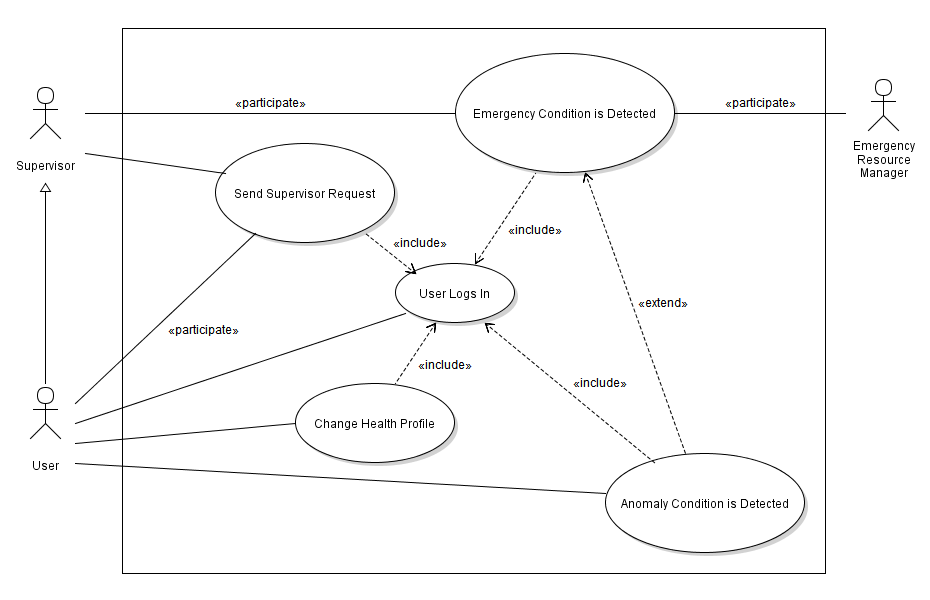
\includegraphics[scale=1.1]{Images/UML/ASOS_usecase}
\end{center}


%\subsubsection{Data4Help Sequence Diagrams}
{\color{Blue}\subsubsection{Data4Help Sequence Diagrams}}

\textbf{Register Device}\par
\begin{center}
	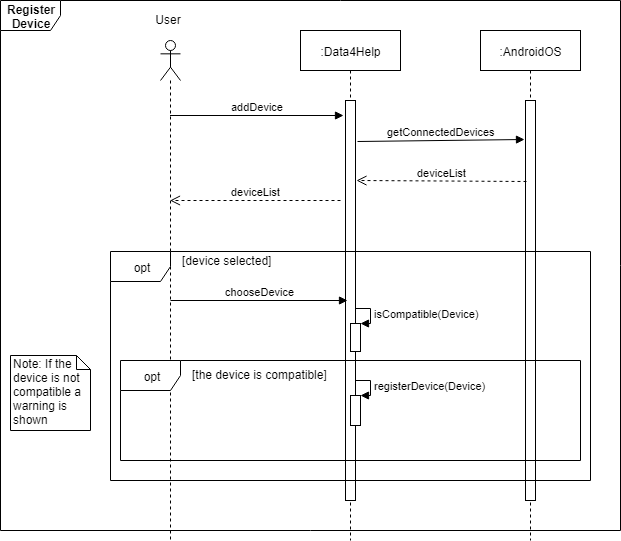
\includegraphics[scale=0.6]{Images/UML/RegisterDeviceSeq.png}
\end{center}

\textbf{Make Request}\par
\begin{center}
	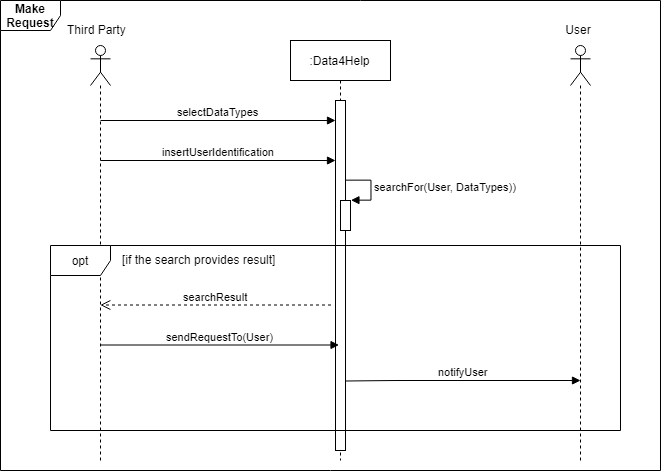
\includegraphics[scale=0.6]{Images/UML/MakeRequestSeq.png}
\end{center}

\textbf{Evaluate Request} \par
\begin{center}
	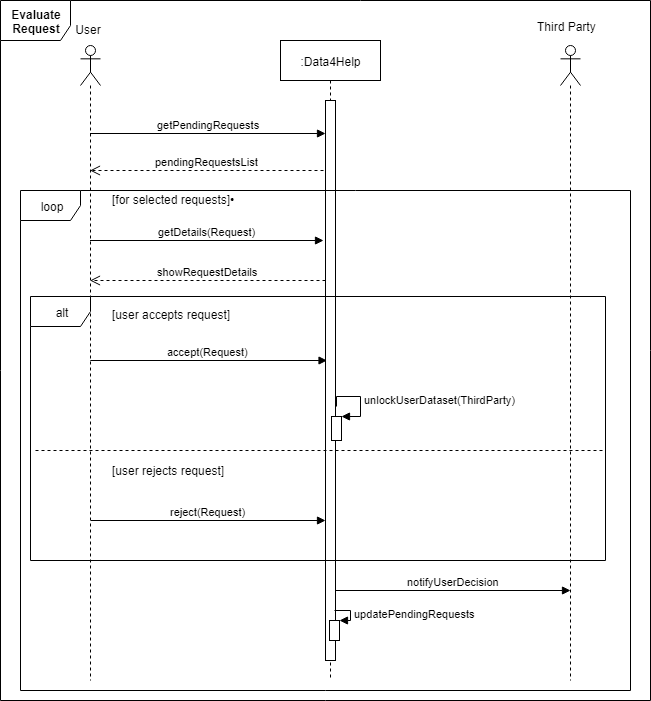
\includegraphics[scale=0.6]{Images/UML/EvaluateRequestSeq.png}
\end{center}

%\subsubsection{AutomatedSOS Sequence Diagrams}
{\color{Blue}\subsubsection{AutomatedSOS Sequence Diagrams}}

\textbf{Emergency Condition is Detected}\par
\begin{center}
	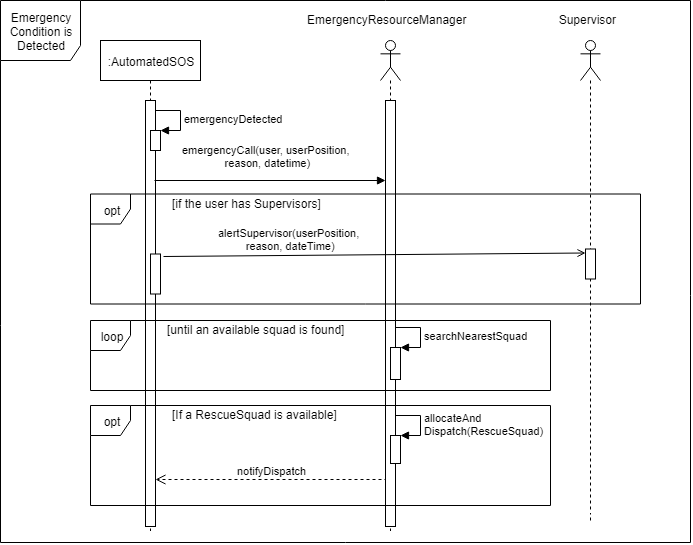
\includegraphics[scale=0.6]{Images/UML/EmergencyConditionsSeq.png}
\end{center}










\
%\subsection {Performance Requirements}
{\color{Blue}\subsection{Performance Requirements}}

Both d4h and asos aim to help the highest number of people. asos must guarantee that the information of the users are sent in real time to the application so the emergency can be solved as soon as possible. A delay higher than 3 seconds can’t be tolerated. D4h have to rendere disponibili the information of each user during an entire month.
\paragraph{}


%\subsection{Design Constraints}
{\color{Blue}\subsection{Design Constraints}}

%\subsection{Software System Attributes}
{\color{Blue}\subsection{Software System Attributes}}
%\subsubsection{Reliability}
{\color{Blue}\subsubsection{Reliability}}
D4H presents a critical factor related to the data processing on server side. As already motivated, this huge amount of information related to each connected user should be processed in real-time especially when supporting ASOS users, any failure of both the services could potentially lead to the death of a person. A domino effect, in which a generic fail may cause the blackout of the entire service is unacceptable and must be avoided.
\paragraph{}

%\subsubsection{Availability}
{\color{Blue}\subsubsection{Availability}}
The software has to be online 24/7, in particular the ASOS part because its chore is to guarantee a constant control of the users, in this case the system should be kept down for the least time possible, for performing maintenance. For minimizing the risk of having interruption of service for patients who need assistance, an availability of at least 99.999\% has to be granted. It is an exigent but required value. Since ASOS relies on D4H for collecting data, both the services should have the same availability. Unfortunately this requirement is too much expensive for all the users of D4H. It is sufficient to provide such level of availability only for all the users who rely on ASOS and an value of 99.99\% for the remaining ones, this solution can reduce appreciably the costs of maintenance.
\paragraph{}

%\subsubsection{Security}
{\color{Blue}\subsubsection{Security}}
Companies and organizations that want to rely on the service must certificate their identity. For the first version of the application, a third party has to provide to the service a valid digital certification, released by a well-known and reliable Certification Authority. This represent an essential security requirement to also provide a strong encrypted communication between the third party and TrackMe. Since TrackMe is also provided with a digital certification, user data sent to the server are encrypted using TLS (Transport Layer Security). \par
Passwords of both users and third parties, must be hashed and salted on server side.
\paragraph{}

%\subsubsection{Maintainability}
{\color{Blue}\subsubsection{Maintainability}}

Especially for D4H, the system will deal with an enormous amount of data coming from a wide variety of sensors, maintainability challenges will concern mainly with the support of new sensor devices appearing in the market that must be supported by the system. The architecture should facilitate the introduction of new products to speed up updated versions of the system.
\paragraph{}

%\subsubsection{Portability}
{\color{Blue}\subsubsection{Portability}}

The application have to be developed in order to support all the android devices with an API level higher or equal to 15 (Android 4.0, Ice Cream Sandwich).





%------------------------------------------------------------------------------------------------------------------------------------------------
\clearpage
{\color{Blue}{\section{Formal Analysis Using Alloy}}}
\label{sect:alloy}
%Organize this section according to the rules defined in the project description. 
\setlength{\parskip}{0.3cm}

The target of this part is to provide a formal model of the software to be, that can be analyzed and tested. Such study is carried out in the Alloy envinronment.  Defining all the aspects of the system is not so trivial in this case, the two services, as said are not independent. ASOS uses a subset of data collected through Data4Help in order to evaluate the user condition, such data are provided by devices registered to D4H, to just name a few.
So in order to not complicate too much the model, only the following  cases are highlighted and tested to facilitate the comprehension:
\par
\textbf{Data4Help}

\begin{itemize}[topsep=-0.1cm]
	\item A third party can access a specific user dataset, only after the same user accepts such request. 
	\item A third party is provided with an anonymous dataset (Anonymous Request) if the number of anonymous users involved in an anonymous request is at least 1000. 
	\item A user dataset is composed only with data provided by registered sensor devices
\end{itemize}

\textbf{AutomatedSOS}
\begin{itemize}
	\item If an emergency condition is detected the nearest ERM is alerted
	\item Anomaly conditions can turn into emergencies only if expressed by the user or after the prevention timeout expires. The reverse conversion is not allowed. Emergency conditions can be directly triggered by critical trigger events (criticality = true).
	\item A user can have a supervisor which is notified each time an anomaly or emergency condition is detected by the system
\end{itemize}


%\section{Alloy Code}
{\color{Blue}{\subsection{Alloy Code}}}
%\subsection{Signatures}
{\color{Blue}{\subsubsection{Signatures}}}
\lstinputlisting[language=alloy]{alloy_code/signatures.als}

%\subsection{Facts and Asserts}
{\color{Blue}{\subsection{Facts and Asserts}}}
\lstinputlisting[language=alloy]{alloy_code/facts_asserts.als}

%\subsection{Predicates}
{\color{Blue}{\subsubsection{Predicates}}}
\lstinputlisting[language=alloy]{alloy_code/predicates.als}

%\subsection{Testing}
{\color{Blue}{\subsubsection{Testing}}}
\lstinputlisting[language=alloy]{alloy_code/testing.als}

\begin{figure}[htp!]
	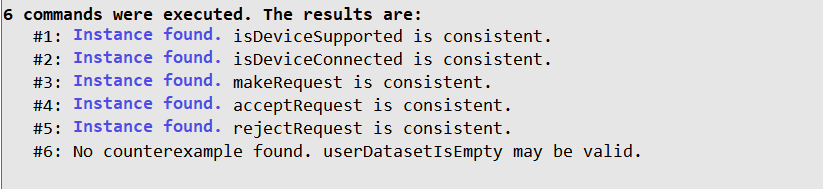
\includegraphics[scale=0.8]{Images/alloy/D4H_consistency.png}
	\captionsetup{justification=raggedright, singlelinecheck=false}
	\vspace*{-2mm}\caption{Consistency Test of D4H model}
	\label{figure17}
\end{figure}
\begin{figure}[htp!]
	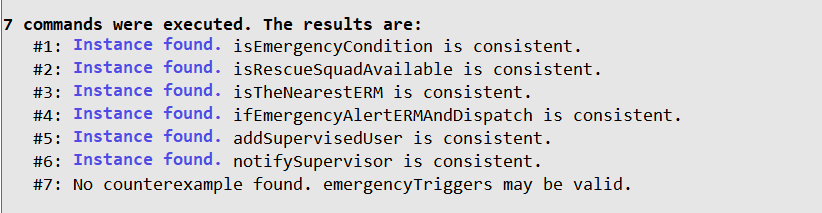
\includegraphics[scale=0.8]{Images/alloy/ASOS_consistency.png}
	\captionsetup{justification=raggedright, singlelinecheck=false}
	\vspace*{-2mm}\caption{Consistency Test of ASOS model}
	\label{figure18}
\end{figure}
\newpage
{\color{Blue}{\subsubsection{Data4Help World}}}
%\subsection{Data4Help World}
\begin{figure}[H]
	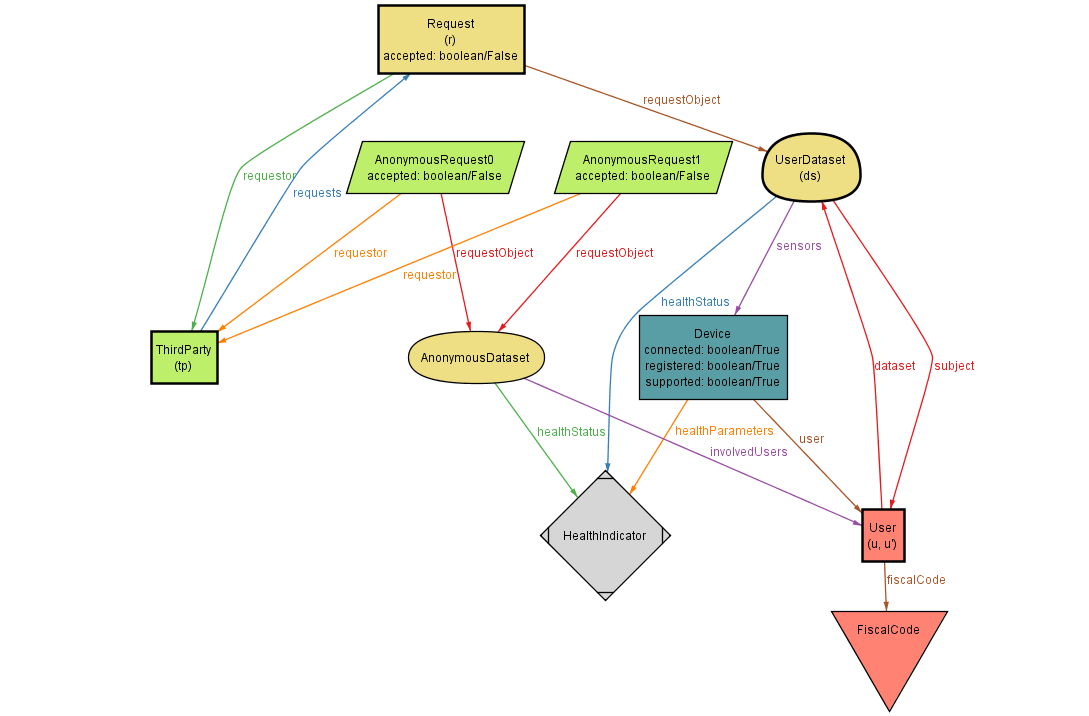
\includegraphics[scale=0.42]{Images/alloy/D4H_world.png}
	\vspace*{-3mm}\caption{Data4Help world generated after testing}
	\label{figure19}
\end{figure}


%\subsection{AutomatedSOS World}
{\color{Blue}{\subsubsection{AutomatedSOS World}}}

\begin{figure}[H]
	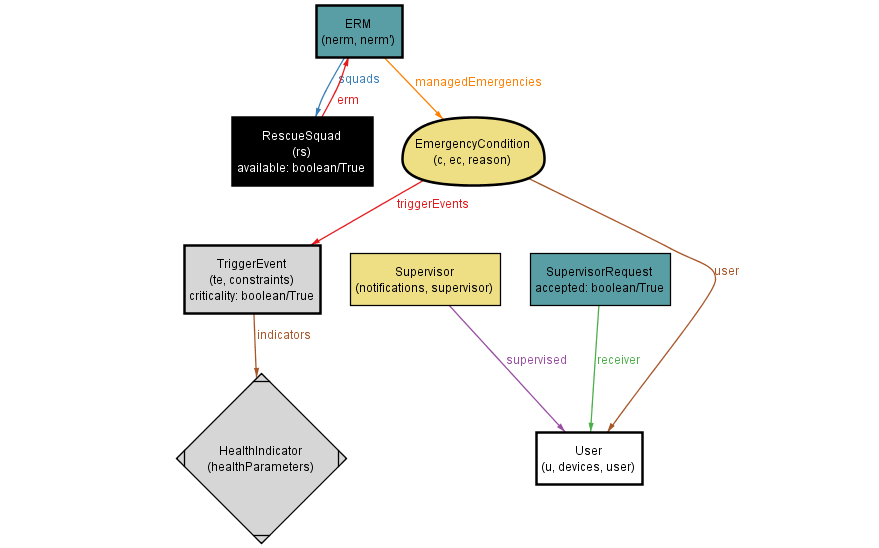
\includegraphics[scale=0.45]{Images/alloy/ASOS_world.png}
	\vspace*{-2mm}\caption{AutomatedSOS world generated after testing}
	\label{figure20}
\end{figure}










%------------------------------------------------------------------------------------------------------------------------------------------------
\clearpage
{\color{Blue}{\section{Effort Spent}}}
\label{sect:effort}
Here is the effort spent by each group member in working at this document.

\begin{table}[H]
\begin{tabular}{|l|c|}
\hline
\textbf{Barbara Ferretti} & \multicolumn{1}{l|}{\textbf{Hours}} \\ \hline
User Interfaces                     & 5                                   \\ \hline
Implementation, Integration and Test Plan & 4 \\ \hline
General  & 3 \\ \hline
\end{tabular}
\end{table}

\begin{table}[H]
	\begin{tabular}{|l|c|}
		\hline
		\textbf{Giorgio Cozza} & \multicolumn{1}{l|}{\textbf{Hours}} \\ \hline
		Introduction & 2 \\ \hline
		Architectural Design & 20 \\ \hline
		Implementation, Integration and Test Plan & 3 \\ \hline
	\end{tabular}
\end{table}




%------------------------------------------------------------------------------------------------------------------------------------------------
%\clearpage
%\addcontentsline{toc}{section}{References}
%\bibliographystyle{plain}
%\bibliography{main}
%------------------------------------------------------------------------------------------------------------------------------------------------




\end{document}
